\documentclass{article}
\usepackage{amsmath}
\usepackage{amssymb}
\usepackage{graphicx}
\usepackage{hyperref}
\usepackage[version=4]{mhchem}


\begin{document}
\section*{Problem}
As shown in the figure, \(A D\) and \(B E\) are the heights of \(\triangle A B C\) and they meet at \(H\). Extend \(A D\) to meet the circumcircle \(O\) at \(G\). Prove: \(H D=D G\).\\
\centering
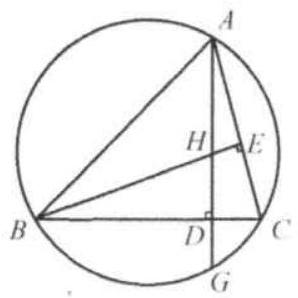
\includegraphics[width=\textwidth]{images/206.jpg}

\section*{Solution}
Connect \(B G\).\\
Since \(B E\) and \(A D\) are the heights, \(\angle H E C=\angle A D C=90^{\circ}\).


Thus points \(C, D, H\), and \(E\) are concyclic. Therefore,\\
\(\angle B H D=\angle B C E=\alpha\).\\
Note that \(\angle A G B=\angle A C B\) (they face the same arc \(A B\) ).\\
That is, \(\angle B G H=\angle B H G=\alpha\).\\
Triangle \(B H G\) is an isosceles triangle and \(B D\) is the perpendicular bisector of \(H G\) and \(H D=D G\).\\
\centering
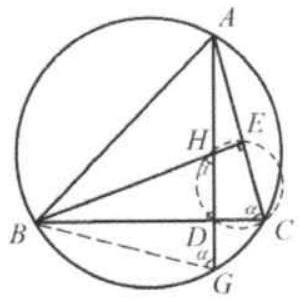
\includegraphics[width=\textwidth]{images/210.jpg}

\end{document}
